%\chapter{Introducción histórica}
%
%\section{Antecedentes históricos y actualidad (español)}
%Primera sección.
%
%\section{Historical and current background (English)}
%
%\begin{otherlanguage}{british}
%En inglés
%\end{otherlanguage}

\chapter{Introducción}

\section{Sistemas ciberfísicos}
Los sistemas ciberfísicos son un tipo especial de sistemas en tiempo real que combinan un micro controlador o programa software, representado mediante una máquina de estados discretos, con uno o varios sensores que interactúan sobre una variable física. Ejemplos de este tipo de entornos son los ordenadores de a bordo que regulan la velocidad de crucero de un vehículo, o el piloto automático que controla la altitud y trayectoria de un avión.

Garantizar el correcto funcionamiento de estas plataformas es crucial, ya que un mal funcionamiento conlleva una reducción del comfort por parte de los usuario o, incluso, la pérdida de vidas humanas. Una manera de asegurarlo es mediante el uso de técnicas de verificación formal. Las técnicas de verificación en tiempo de ejecución \cite{STTT_RV_21} (\emph{runtime verification} en inglés) implementan un monitor que supervisa que la ejecución actual cumple con los requisitos especificados. Los monitores actúan como guardianes, alertando al usuario cuando la ejecución se desvía del comportamiento deseado e, incluso, implementando contramedidas para revertir ese hecho y redirigir el sistema hacia un estado saludable. 

Existen diversos formalismos para definir los comportamientos deseados y no deseados. Los requisitos se pueden expresar operacionalmente, mediante algún tipo de autómata de estados finito, o declarativamente, mediante una descripción lógico-matemática. Dentro de esta segunda categoría, la lógica temporal es un tipo de lógica modal que expresa propiedades sobre un \emph{estado} en particular del sistema, o sobre los \emph{caminos} (es decir, secuencia de estados) que atraviesa. En este trabajo utilizaremos Signal Temporal Logic \cite{STL}, un tipo de lógica temporal enfocada al análisis de señales analógicas o reales.

\section{Lógica Temporal}

Si navegamos por internet o buscamos en los libros acerca de qué es la lógica temporal tarde o temprano daremos con una cita del filósofo alemán Kant que cita: 

\begin{center}
\textit{"la posibilidad de principios apodícticos de las relaciones del tiempo, o axiomas del tiempo en general. Tiene una sola dimensión: los distintos tiempos no son simultáneos, sino sucesivos"}
\end{center}

Y, aunque quizás sacado de todo contexto, es un buen primer comienzo para explicar acerca de qué es el tiempo y por consiguiente qué tiene que ver la lógica con éste. Y es que Kant quería expresar que el tiempo es algo que va ocurriendo constantemente, es un conjunto de hechos que juntos transcurren en una dirección y conforman el tiempo, pues bien, teniendo en cuenta esta idea podemos llegar a comprender y diferenciar la lógica temporal. 

La lógica proposicional no tiene la persepción de tiempo, en este tipo de lógica tenemos hechos que son verdaderos o falsos, que unidos pueden transformarse en verdad o no, pero nunca individualmente cambian su valor, por ejemplo si decimos que:

\begin{center}
s = ``El día está soleado''
\end{center}

Este argumento será eterno individualmente, aún asi realicemos operaciones con él como negarlo $\neg{s}$, todo el argumento se verá afectado en todo momento:

\begin{center}
$\neg{s}$ = ``El día no está soleado''
\end{center}

Pero como todos podemos percibir, en la realidad esto no sucede, en otras palabras, puede que "no todo el día esté soleado", quizás si por la mañana y no por la tarde o visceversa, esto es lo que trata de expresar la lógica temporal. En un momento determinado una expresión puede ser verdad mientras que en otra hora, minuto, segundo, o cuálquier otra unidad que utilicemos para medir el tiempo , puede cambiar y tener un valor diferente. 

\section{Objetivos}

Los objetivos de este proyecto son:

\begin{itemize}
\item extender las capacidades de la lógica temporal STL para expresar propiedades que involucren \textit{tendencias} (derivadas), o \textit{acumulaciones} (integrales),    
\item implementar esos nuevos operadores lógicos en las herramientas software actuales; y, por último,
\item proporcionar una interfaz de usuario amigable que facilite la interacción con dichas herramientas.  
\end{itemize}

En particular, los objetivos de proyecto se han plasmado en contribuciones concretas sobre las siguientes herramientas software preexistentes:

\begin{itemize}
\item \textbf{STLEval} \cite{StlEval}: Es una herramienta capaz de procesar especificaciones en STL y evaluarlas sobre una señal real. Ha recibido la implementación de los nuevos operadores lógico temporales que calculan derivadas e integrales sobre una señal.
\item \textbf{ParetoLib} \cite{ParetoLib}: Es una biblioteca de de minería que aprende las configuraciones (in)válidas del sistema monitorizado, expresadas como plantillas o especificaciones paramétricas en STL. ParetoLib internamente se conecta con STLEval para la ejecución de los cálculos. Ha recibido una actualización de los binarios y bibliotecas DLL de STLEval que empaqueta de forma conjunta con el resto de la biblioteca, así como la interfaz gráfica de usuario. La nueva interfaz gráfica de usuario permite interaccionar tanto con la biblioteca de aprendizaje como indirectamente con la herramienta STLEval.
\end{itemize}

\section{Organización del documento}

El documento está dividido en 4 capítulos. En el capítulo \ref{cha:stl} detallaremos la semántica e implementación de los nuevos operadores lógicos. El capítulo \ref{cha:gui} está dedicado a la nueva interfaz gráfica de usuario. Finalmente, continuamos con las conclusiones más relevantes del proyecto en el capítulo \ref{cha:concl}, donde se incluye también ideas para el trabajo futuro. %Los anexos X recogen imágenes, código adicional, $\ldots$.

\section{Planificación temporal y esfuerzo}

Este proyecto tuvo una duración de 8 meses y ha sido realizado por dos estudiantes a tiempo parcial, Dmytro Vernyuk (GII) y Javier Romero Flores (GIC), con una dedicación media de 3 horas al día. Los alumnos han estado tutorados por José Ignacio Requeno mediante reuniones semanales. Se han modificado o creado aproximadamente 1300 líneas de código, que están repartidas entre las dos herramientas software actualizadas y la nueva interfaz gráfica de usuario. El código desarrollado en este proyecto puede consultarse en ramas dedicadas a las nuevas funcionalidades de los correspondientes repositorios web (rama \textit{derivative} de STLEval y rama \textit{GUI} de ParetoLib). El proyecto arrancó el 13 de septiembre del 2021, ha durado 8 meses y ha constado de 4 fases.

\subsection{Primera - Investigación}
El proyecto se inició con una primera fase de investigación, donde nos dedicamos a adquirir los conocimientos teóricos necesarios para el trabajo: leer información sobre qué es la lógica temporal y la principal diferencia con otras lógicas modales. Recurrimos tanto al material proporcionado por el instructor como al material externo disponible para aprender las principales definiciones y sintaxis básicas. 

Ésta fue la parte más complicada de todo el trabajo no sólo por la dificultad teórica de la información especializada en el ámbito de la verificación, sino también por el cambio de paradigma que supone comprender el concepto principal de ésta lógica: que una afirmación se puede convertir en negación dependiendo del instante en el que se evalúa la expresión.
	
\subsection{Segunda - Documentación}

	Después de adquirir los conocimientos teóricos previos necesarios para la comprensión de las funcionalidades a implementar, continuamos con la lectura de la documentación de las bibliotecas y herramientas software que debíamos extender: su arquitectura software y jerarquía de clases. Dedicamos gran parte del esfuerzo a estudiar la definición de los operadores de derivación e integración propuestos en la literatura científica, y su posterior codificación e incorporación a la herramienta software STLEval.
	
	En esta fase, nuestra mayor dificultad fue 1) la labor de aprendizaje de la estructura interna del código de STLEval, y 2) la adquisición y aplicación de las nociones de derivación e integración sobre señales temporales.

\subsection{Tercera - Implementación}

	Implementamos las operaciones de derivación e integración de señales temporales en la herramienta software STLEval. Completamos esta tarea con un conjunto de pruebas sobre señales temporales con características \textit{benignas} que nos facilitaron ejecutar tests de validación: por ejemplo, la integral de una señal periódica (sinusoidal o triangular) simétrica sobre el eje horizontal debe ser cero en determinados intervalos.

\subsection{Cuarta - Diseño y Finalización}

	Como última tarea implementamos la interfaz gráfica de la aplicación, partiendo de un primer boceto que estabilizamos al cabo de dos reuniones. La tarea más complicada de este proceso fue la conexión entre los diferentes componentes de la interfaz con los métodos propios de las herramientas STLEval y ParetoLib, que ejecutan toda la lógica del programa.
	
	La conexión con STLEval se realizó mediante una API preexistente en C++ que ya estaba integrada en Python a través de la biblioteca ParetoLib. Este hecho, la posibilidad de acceder tanto a la biblioteca de minería ParetoLib como indirectamente a la herramienta STLEval, motivó la elección de Python como lenguaje de programación para el diseño de las ventanas de usuario. La facilidad de uso del lenguaje así como la cantidad de bibliotecas auxiliares para el tratamiento de datos con las que extender las funcionalidades de la interfaz en el futuro contribuyeron también a esta decisión.
	


\section{Organización de Equipo}

Debido a la dificultad teórica de este proyecto, decidimos realizar las tareas de manera conjunta: todos los apartados de este proyecto a excepción de la labor de documentación se realizaron a la par por ambos integrantes del equipo. 

La planificación coincide con las fases del proyecto, indicamos las fechas exactas en el siguiente gráfico.

\begin{figure}
\centering
  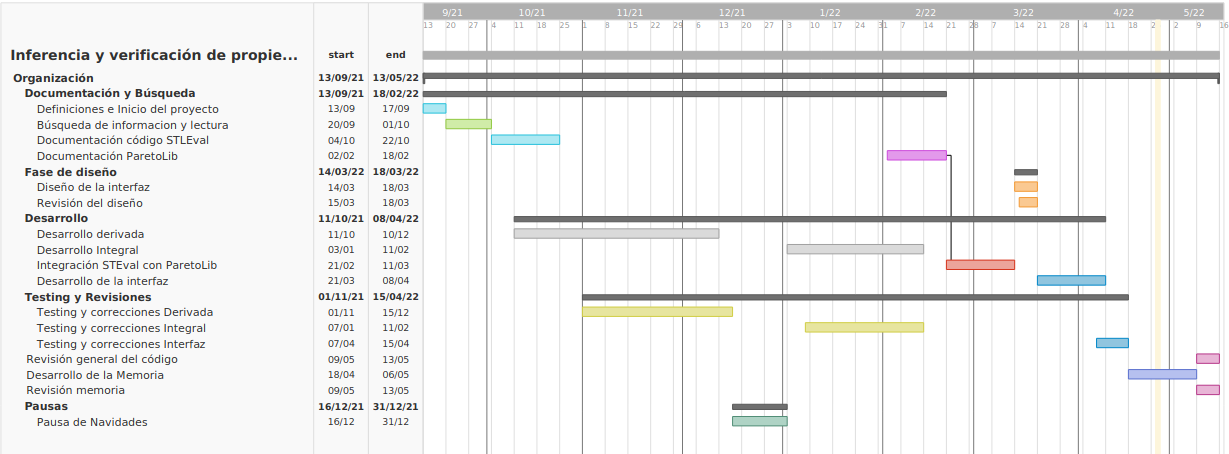
\includegraphics[width=.9\linewidth ,angle = 90,scale = 1.2]{images/gant}
\caption{Diagrama de Gantt.}
\label{fig:gant}
\end{figure}
